\documentclass{article} % \documentclass{} is the first command in any LaTeX code.  It is used to define what kind of document you are creating such as an article or a book, and begins the document preamble

\usepackage{amsmath} % \usepackage is a command that allows you to add functionality to your LaTeX code
\usepackage{graphicx}
\graphicspath{ {./images/} }
\title{Discrete Time Signals and Systems} % Sets article title
\author{Hunter Mills} % Sets authors name
\date{\today} % Sets date for date compiled

% The preamble ends with the command \begin{document}
\begin{document} % All begin commands must be paired with an end command somewhere
    \maketitle % creates title using information in preamble (title, author, date)
    
    \section{Sampling and Reconstruction of Signals} % creates a section
    These notes only cover 6.1, 5.3 and 6.5.1.\\
    
    This chapter will cover time-domain signaling, A/D conversion and D/A conversion. It also covers the sampling of signals that are characterized as bandpass signals. 
    
    \subsection{Ideal Sampling and Reconstruction of CT Signals}
    To produce a DT signal from a CT signal it must be converted to a sequence of numbers. It is normally done by sampling the analog signal periodically, 
    \begin{equation}
	x(n) = x_a(nT), \;\;\; -\infty < n < \infty
	\end{equation}
    This describes the sampling process in the time domain, with the sampling frequency $F_s = 1/T$. $F_s$ must be large enough such that the sampling does not cause any loss of spectral information. In order to determine the relationship between the spectrum of the DT signal and the analog signal, 
    \begin{equation}
	t = nT = \frac{n}{F_s}
	\end{equation}
	It can be derived (in the book pg 386) that
	\begin{equation}
	\int_{-1/2}^{1/2}X(f)e^{j2\pi fn}df = \int_{-\infty}^{\infty}X_a(F)e^{j2\pi nF/F_s}dF
	\end{equation}
	which produces the relationship
	\begin{equation}
	f = \frac{F}{F_s}
	\end{equation}
	The book concludes that 
	\begin{equation}
	X(F) = F_s \sum_k X_a(F-kF_s)
	\end{equation}
	or 
	\begin{equation}
	X(f) = F_s \sum_k X_a[(f-k)F_s]
	\end{equation}
	This is the desired relationship between $X(F)$ or $X(f)$ of the DT signal and the spectrum $X_a(F)$ of the analog signal. The right hand side of the previous two equations is a periodic repetition of the scaled spectrum with period $F_s$. This periodicity is necessary because $X(f)$ is periodic with the period $f_p = 1$ or $F_p = F_s$. If the sample rate is 2x the highest frequency in a bandlimited signal there will be no aliasing. If the sampling frequency $F_s$ is selected such that $F_s \ge 2B$ where $2B$ is the \textit{Nyquist Rate} then
	\begin{equation}
	X(F) = F_s X_a(F), \;\;\; |F| \le F_s/2
	\end{equation}
	A digital signal can be reconstructed using the following formula,
	\begin{equation}
	x_a(t) = \sum_n x_a(nT) \frac{\sin (\pi /T)(t-nT)}{(\pi /T)(t-nT)}
	\end{equation}
	This formula is an interpolation formula for reconstructing $x_a(t)$ from its samples. It consists of the sampled functions and a sinc function. The relationship of the sampled spectrum and the analog spectrum is shown in the following figure. 
   
	\begin{figure}[h]
	\centering
	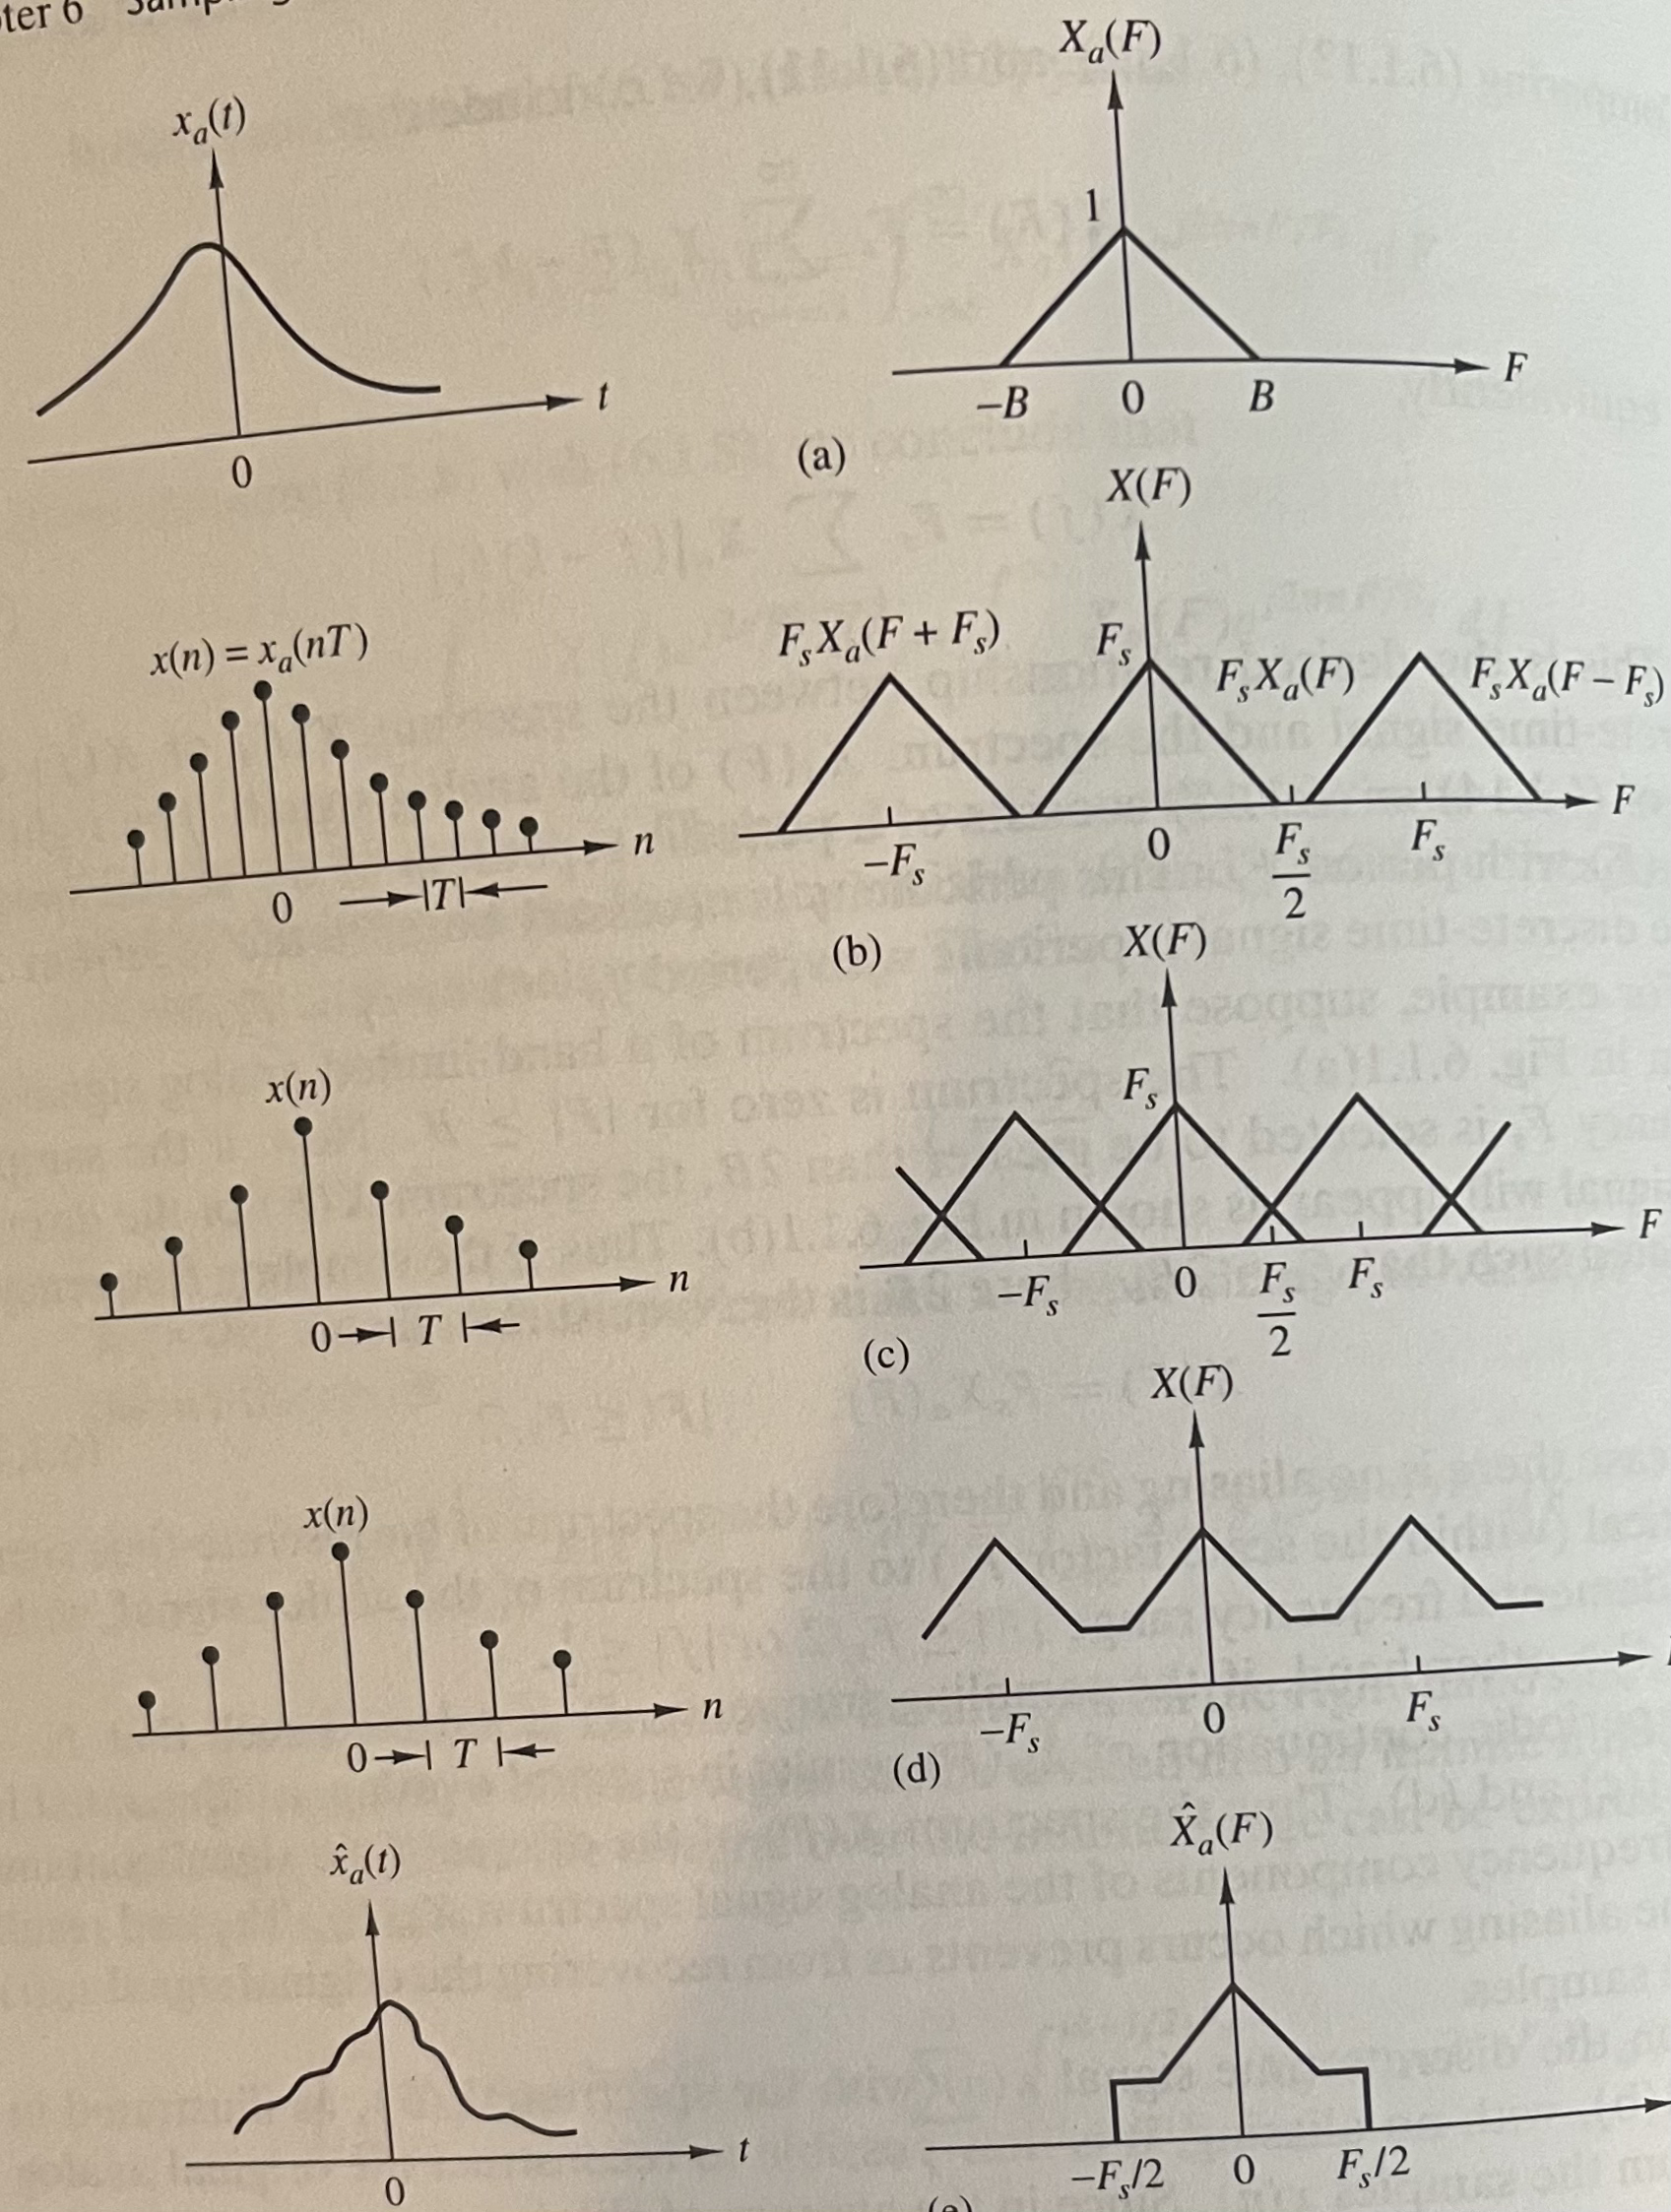
\includegraphics[width=5cm]{spectrum}
	\caption{Sampled Spectrum's}
	\end{figure}
	\textbf{Sampling Theorem}\\
	
	A bandlimited CT signal with highest frequency B Hz can be uniquely recovered from its samples provided that the sample rate $F_s \ge 2B$ samples per second. When aliasing occurs due to too low of a sample rate, the effect can be described by a multiple folding of frequency axis of $F$ for the analog signal.
	
	\begin{figure}[h]
	\centering
	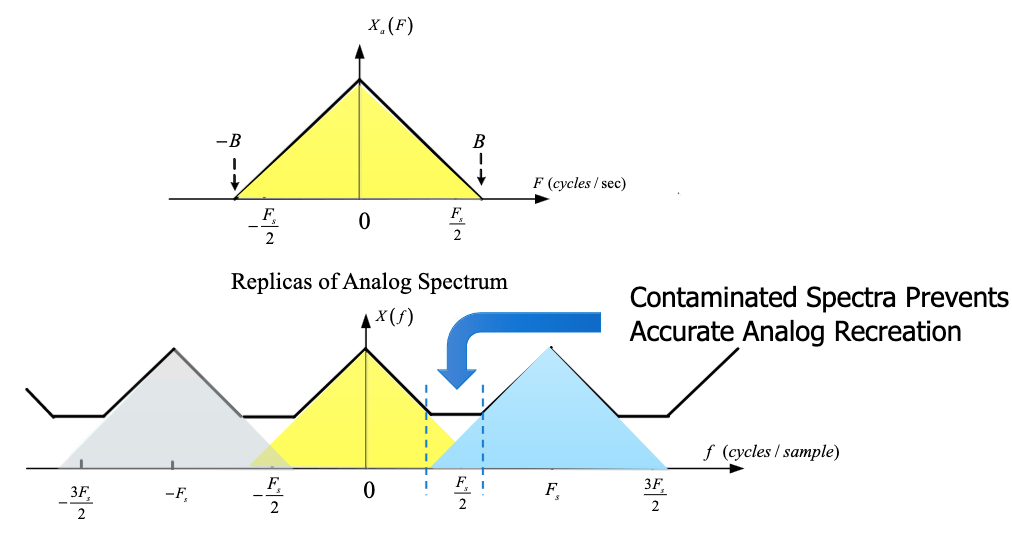
\includegraphics[width=10cm]{aliasing}
	\caption{Aliasing occurs when $F_s < 2B$}
	\end{figure}
	
	\subsection{Analog-to-Digital and Digital-to-Analog Converters}
	In the previous chapters, these notes have looked at digital singals that have been ideal. We have assumed no quantization error and round off errors being negligible. \\
	\textbf{Analog-to-Digital Converters}\\
	
	When converting a signal from analog to digital, we will have to quantize the sampled values to a finite number of levels and represent each level by a number of bits. In practice, the sampling of a CT signal is done by a sample and hold circuit. The sampled signal is then quantized and converted to digital form. Some errors that the sample and hold circuit can cause is \textit{jitter} which is difference in the sample period and changes in the voltage held during conversion. \\
	\textbf{Quantization and Coding}\\
	
	The basic task of the quantizer is to take the continuous voltage amplitude into a discrete set of digital code words. Quantization is nonlinear and noninvertible process that maps a given amplitude $x(n) = x(nT)$ at time $t = nT$ into an amplitude $x_k$ taken from a finite set of values. 
	
	\begin{figure}[h]
	\centering
	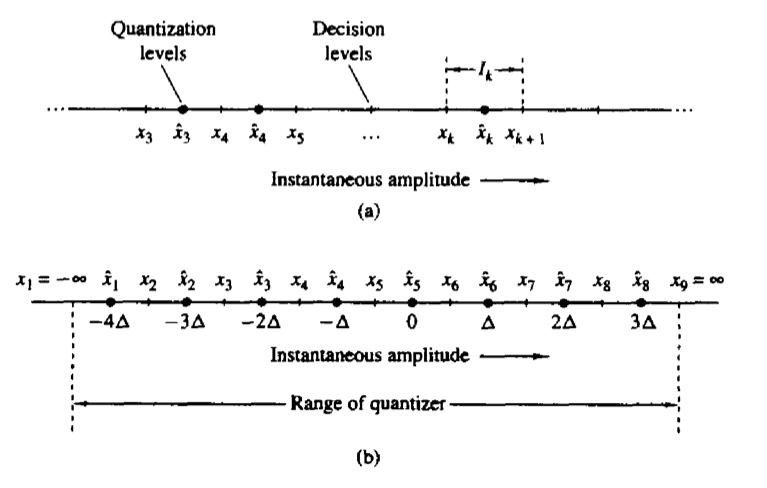
\includegraphics[width=10cm]{quant}
	\caption{Quantization}
	\end{figure}
	In most DSP systems the process is independent of $n$ (memoryless) and it is uniform quantizers where
	\begin{equation}
	\hat{x}_{k+1} - \hat{x}_k = \Delta
	\end{equation}
	\begin{equation}
	x_{k+1} - x_k = \Delta
	\end{equation}
	where $\Delta$ is the step size. If zero is assigned a quantization level then it is the \textit{midtread type} and if zero is assigned a decision level then it is a \textit{midrise type}. The medtread type is preferred over midrise. The quantization error $e_q(n)$ is always in the range,
	\begin{equation}
	-\frac{\Delta}{2} < e_q(n) \le \frac{\Delta}{2}
	\end{equation}
	
	The coding process in an A/D converter assigns a unique binary number to each quantization level. 
	
	\begin{figure}[h]
	\centering
	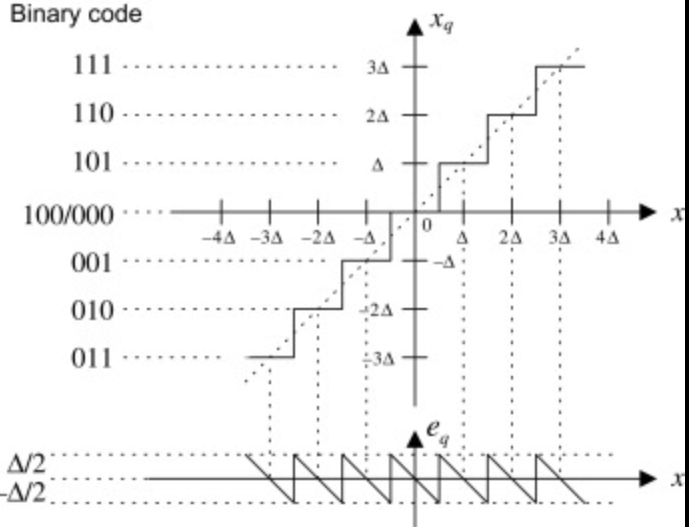
\includegraphics[width=10cm]{ch6_quant}
	\caption{Midtread Quantizer}
	\end{figure}
	\textbf{Analysis of Quantization Errors}\\
	
	TO determine the effects of quantization on the performance of an ADC, the book uses a statistical approach. In this model we assume that the quantization error is random in nature and is added to the original signal. If the input signal is within the ADC range, $e_q(n)$ is bounded to $|e_q(n)| < \Delta/2$ and is called granular noise. When the input is outside the ADC range it causes clipping to the max ADC input value. This is modeled as
	\begin{equation}
	x_q(n) = x(n) + e_q(n)
	\end{equation}
	The assumptions of the model are\\
	\textbf{1.} The error $e_q(n)$ is uniformly distributed over the range $-\Delta /2 < e_q(n) < \Delta /2$\\
	\textbf{2.} The error sequence is stationary white noise sequence, ie the error $e_q(n)$ and the error $e_q(m)$ for m != n are uncorrelated \\
	\textbf{3.} The error sequence is uncorrelated with x(n)\\
	\textbf{4.} x(n) is zero mean and stationary.\\
	
	When the $\Delta$ is small and x(n) traverses several quantization levels between successive samples then the signal-to-quantization-noise (power) ratio can be expressed as
	\begin{equation}
	SQNR = 10\log_{10} \frac{P_x}{P_n}
	\end{equation}
	where $P_x$ = $\sigma_x^2 = E[x^2(n)]$ is the signal power and $P_n$ = $\sigma_e^2 = E[e_q^2(n)]$ is the power of quantization noise. If the quantization error is uniformly distributed in the range $(-\Delta /2, \Delta /2)$, the mean value of the error is zero and the variance (quantization noise power) is
	\begin{equation}
	Pn = \frac{\Delta^2}{12}
	\end{equation}
	\begin{equation}
	SQNR = 10\log_{10} \frac{P_x}{P_n} = 20 \log \frac{\sigma_x}{\sigma_e}
	\end{equation}
	\begin{equation}
	SQNR = 6.02b + 16.81 - 20 \log \frac{R}{\sigma_x}dB
	\end{equation}
	where b is the number of bits in the quantizer and R is the range of the ADC. This formula cannot model real life ADC since the fabrication of ADC are not close to the ideal.\\
	\textbf{Digital-to-Analog Converters}\\
	
	In general DAC's are constructed with a Digital-to-analog converter, then a sample and hold, then finally a lowpass smoothing filter. The DAC receives a binary code and outputs a voltage corresponding to the input. An important parameter of a DAC is the \textit{settling time} which is the time required for the output of the DAC to reach and remain within a given fraction of the final value. Often the input code word results in a high amplitude transient called a \textit{glitch}. The usual way to fix this is a sample and hold. The interpolation function of the sample and hold system is a square pulse
	\begin{equation}
	g_{sh}(t) = 
		\begin{cases}
      		1, & \;\;\; 0 \le t \le T \\
      		0, & \text{otherwise}
    	\end{cases} 
	\end{equation}
	And the frequency domain characteristics are
	\begin{equation}
	G_{SH}(F) = T \frac{\sin \pi FT}{\pi FT}e^{-2\pi F(T/2)}
	\end{equation}
	The low pass filter response to smooth the output of the sample and hold is
	\begin{equation}
	H_a(F) = \begin{cases}
      		\frac{\pi FT}{\sin \pi FT}e^{2\pi F(T/2)}, & \;\;\; |F| \le F_s/2 \\
      		0, & \text{otherwise}
    	\end{cases} 
	\end{equation}
	\subsection{Sampling of DT Signals}
	In this section we use the ideas developed for sampling and representation of CT signals to discuss the sampling and reconstruction of lowpass and bandpass DT signals. The approach is to conceptually reconstruct the underlying CT signal and then re-sample at the desired sampling rate. \\
	\textbf{Sampling and Interpolation of DT Signals}
	Suppose x(n) is sampled periodically by keeping every \textit{D}th sample and deleting the (D-1) samples in between. This is called decimation
	\begin{equation}
	x_d(n) = x(nD), \;\;\; -\infty < n < \infty
	\end{equation}
	and the spectrum for $x_d(n)$ is 
	\begin{equation}
	X_d(F) = \frac{1}{DT}\sum_k X_a(F - k\frac{F_s}{D})
	\end{equation}
	\begin{equation}
	X_d(F) = \frac{1}{D}\sum_{k=0}^{D-1} X(F - k \frac{F_s}{D})
	\end{equation}
	To avoid aliasing the sampling rate should satisfy $F_s/D \ge 2B$. In sampling the CT spectrum it is repeated periodically in the discrete frequency domain. In DT the periodic spectrum X(F) is repeated D times to cover one period of the periodic frequency domain. 
	
	\begin{figure}[h]
	\centering
	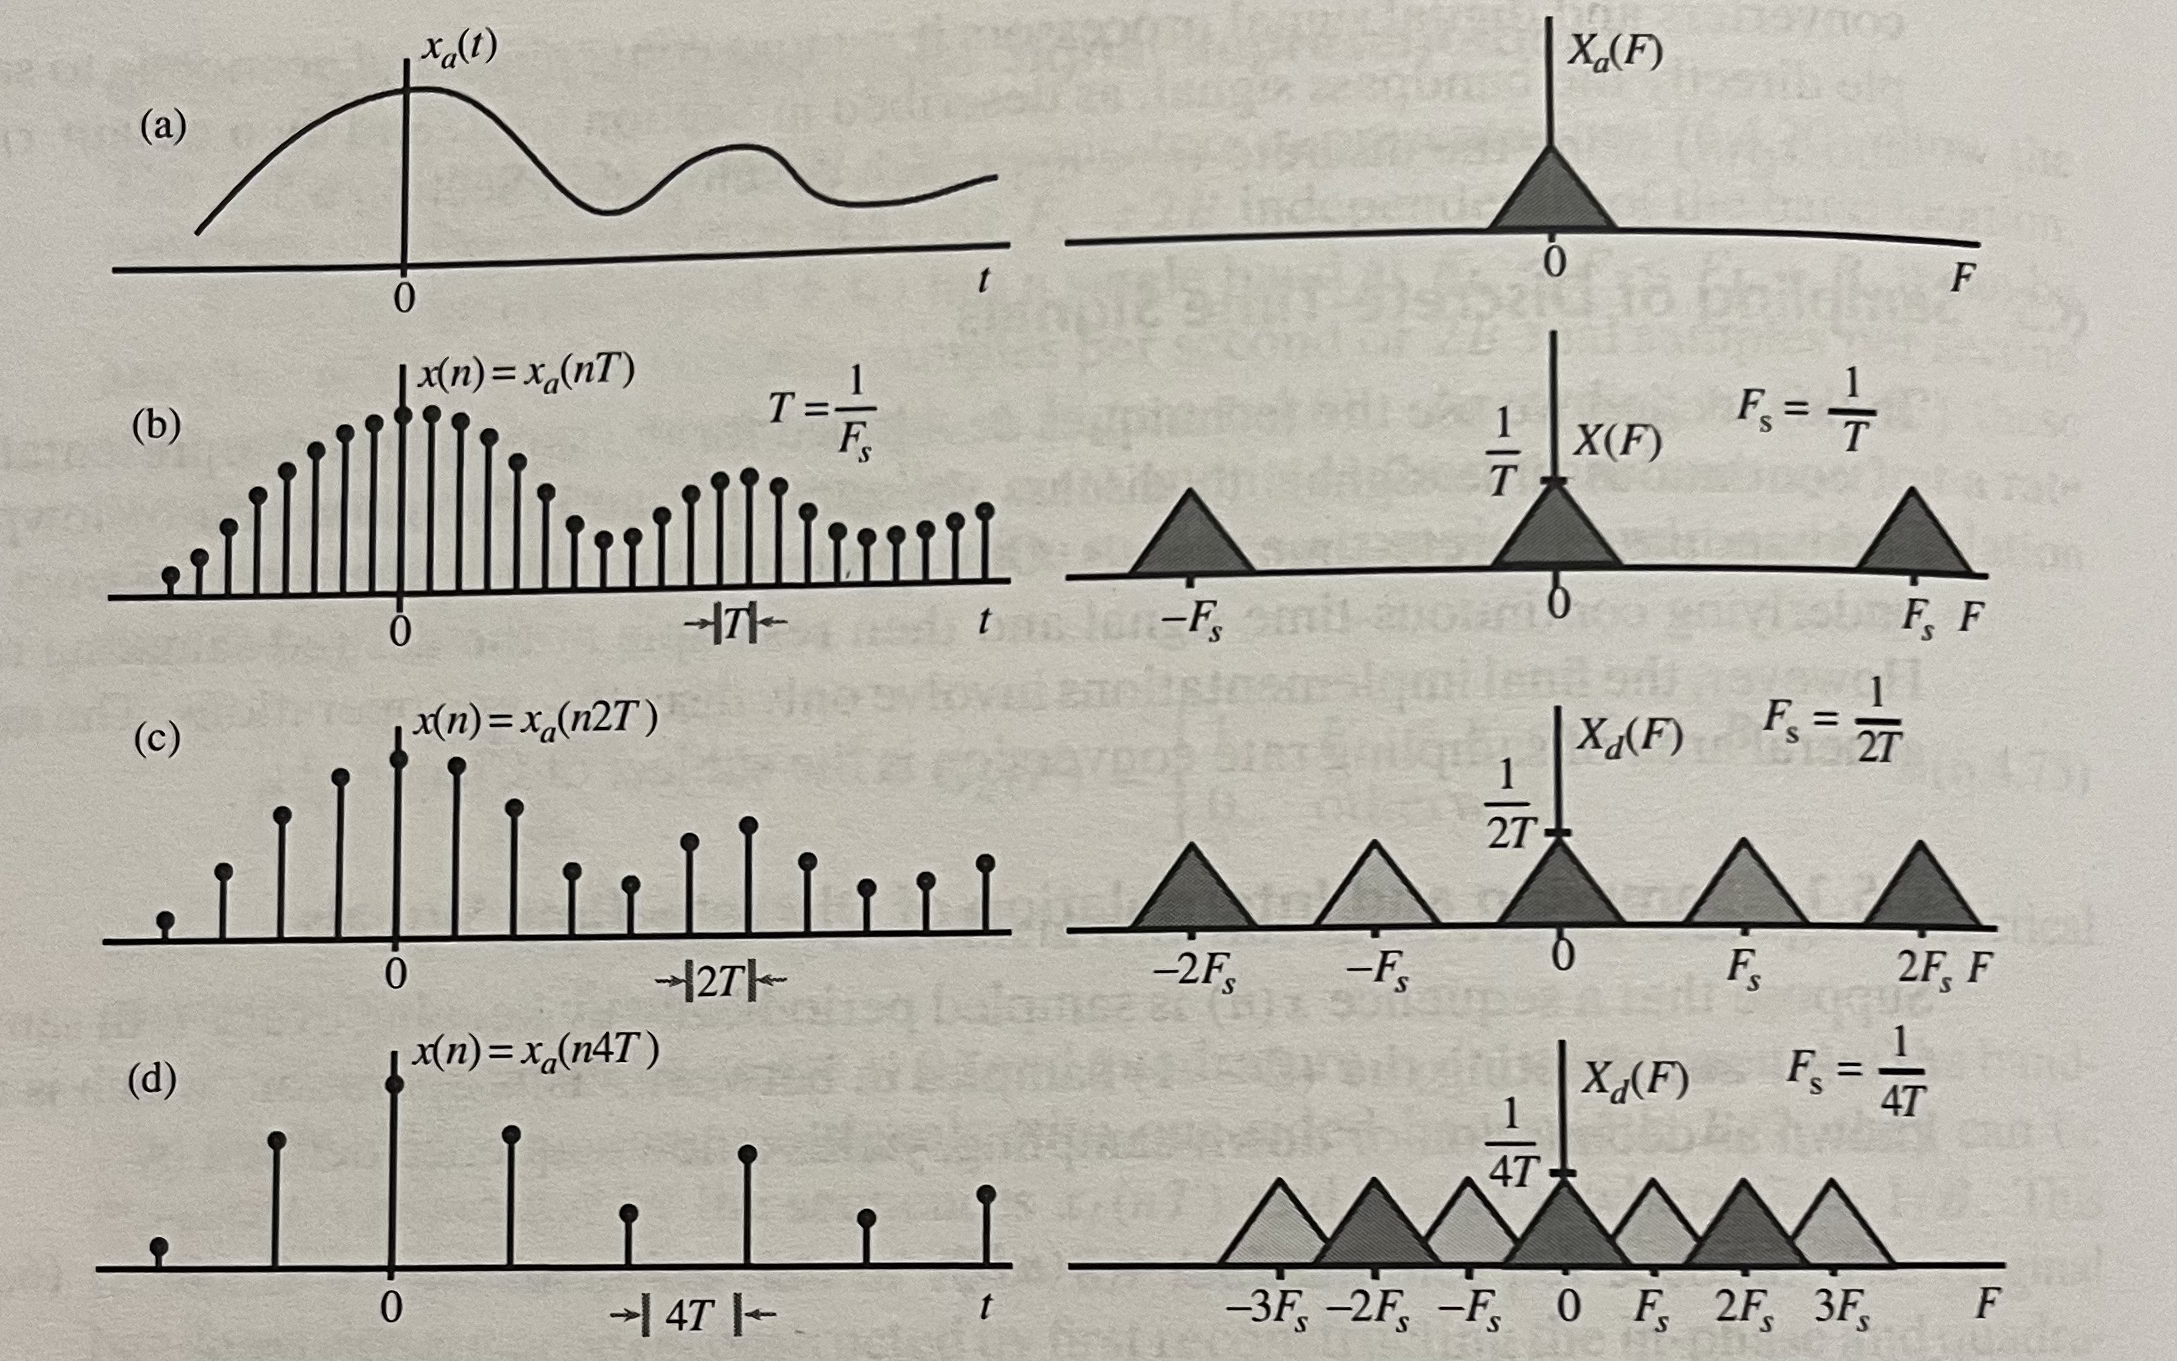
\includegraphics[width=10cm]{downsample}
	\caption{Downsampling in the Frequency Domain}
	\end{figure}
	To reconstruct the original sequence we use
	\begin{equation}
	x(n) = \sum_m x_d(m)\frac{\sin \frac{\pi}{D}(n-mD)}{\frac{\pi}{D}(n - mD)}
	\end{equation}
	This is impractical since the summation is over all m. The DT interpolation formula is
	\begin{equation}
	x_{lin}(n) = \sum_m x(m)g_{lin}(n-mD)
	\end{equation}
	where
	\begin{equation}
	g_{lin}(n) =  \begin{cases}
      		1 - \frac{|n|}{D}, & \;\;\; |n| \le D \\
      		0, & \text{otherwise}
    	\end{cases} 
	\end{equation}
	There is a complex polyphase way to interpolate, but the way discused in this chaper is to instert (D-1) zeros into $x_d(n)$ between samples (which creates $\hat{x}(n)$ and use the formula 
	\begin{equation}
	x(n) = \sum_k \hat{x}(k)g_{lin}(n-k)
	\end{equation}
	Sampling and interpolation of a DT signal essentially corresponds to a change of its sampling rate by an integer factor. 
	
	

\end{document} % This is the end of the document